
\documentclass[10pt,conference]{IEEEtran}

\usepackage[nocompress]{cite}
\usepackage{graphicx}
\usepackage{subfigure}
\usepackage{verbatim}
\usepackage{booktabs}
\usepackage{array}
\usepackage{amsmath}
\usepackage{amsfonts}
\usepackage{amssymb}
\usepackage{bm}
\usepackage{algorithm}

\usepackage[noend]{algpseudocode}

\newtheorem{theorem}{Theorem}
\newtheorem{lemma}[theorem]{Lemma}
\newtheorem{proposition}[theorem]{Proposition}
\newtheorem{corollary}[theorem]{Corollary}
\newtheorem{observation}{Observation}
\newtheorem{definition}{Definition}
\newtheorem{claim}{Claim}

\newcommand{\ignore}[1]{{}}

%\usepackage{color}
%\usepackage{arcs}
\usepackage[usenames,dvipsnames]{color}
\usepackage{colortbl}

\usepackage{url}
\usepackage[colorlinks,linkcolor=blue,anchorcolor=green,citecolor=red, backref]{hyperref}

\usepackage{booktabs}
\usepackage{threeparttable}
\usepackage{multirow}



\begin{document}

\title{differential privacy and machine learning review}

\author{\IEEEauthorblockN{xiang li}\\
\IEEEauthorblockA{\small huazhong university of science and technology, wuhan, china\\
}}


\maketitle

\begin{abstract}
Privacy preserving in data release and mining is a hot topic in the information security field currently.
As a new privacy notion,differential privacy(DP) has grown in popularity recently due to its rigid and provable privacy guarantee.After analyzing the advantage of differential privacy model relative to the traditional ones,this paper surveys the theory of differential privacy and its application on machine learning.We explore the interplay between machine learning and differential privacy, namely privacy-preserving machine learning algorithms and learning-based data release mechanisms. 
\end{abstract}

\begin{IEEEkeywords}
differential privacy, privacy preservation, machine learning.
\end{IEEEkeywords}

\IEEEpeerreviewmaketitle


\section{Introduction}
\label{sec:introduction}

With the continuous popularization and deepening of information technology applications, various information systems have stored and accumulated a wealth of data, such as patient diagnostic data sets established by medical institutions, customer online transaction data collections collected by e-commerce companies, and so on. Analysis can enable people to gain more knowledge about the real world. Therefore, for research institutions, information consulting organizations, and government decision-making departments, data is a very important basic resource. This demand has greatly promoted the release and sharing of data. 

However, the data set usually contains many personal privacy information, such as medical diagnosis results, personal consumption habits, and other data that can reflect personal characteristics, and these information will be leaked along with the release and sharing of data sets. Although deleting the identifier attributes (such as name, ID number, etc.) of the data set can protect personal privacy to some extent, but some attack cases show that this simple operation is far from enough to guarantee the security of private information.

From the perspective of existing research, k-anonymity\cite{Sweeney2012} and its extended models have been widely studied in the field of privacy protection. The basic idea of these models is that the attributes related to the attacker background knowledge are defined as quasi identifiers in the data set. By generalization and compression processing, all the records are divided into several equivalence group, and the records in each of the equivalents have the same quasi identifier, so that a record can be hidden in a set of records. Therefore, such a model is also known as a packet based privacy protection model.

However, follow-up studies have shown that these models have two main defects, which do not provide enough security, and they always need to be perfected because of the emergence of new attacks. For example, to resist "Conformance" attacks, l-diversity\cite{Machanavajjhala2006L}, t-closenes s\cite{Li2007t} and other models have been proposed successively; in these methods, if their sensitive features are the same, the samples are grouped, and if the number of samples in the group is large enough, a group is published. Intuitively, it is very difficult for an attacker to distinguish a single sample. However, these methods can not prevent background attacks. In extreme cases, attackers may know the contents of all rows in the collection. Consider a database that stores four people's addresses and revenues, and uses anonymous to publish private data. If three people live in the same city, the average income of the city and three people is divulged. Now suppose the attacker knows that two people in the database live in Los Angeles, and third people live in New York. If no data were released, the attacker could easily infer that the fourth person lived in Los Angeles.

Therefore, how to protect private information or sensitive information not to be leaked in the learning process has become a very meaningful research topic in the study of machine learning.

In this paper, we first introduce the concept of differential privacy (Section 1), and briefly analyze some important properties of differential privacy. The application of differential privacy in machine learning is introduced later. We mainly introduce these aspects from differential privacy supervised learning (Section 2), differential privacy unsupervised learning (Section 3) and model assessment of differential privacy machine learning (Section 4). Finally, we summarize the current situation and development prospects of differential privacy and differential privacy machine learning, and summarize the existing results.

\section{Differential Privacy}
Differential privacy is a widely used definition of privacy. Intuitively, it is necessary to export information about the underlying dataset, which is robust to any change of a sample, thus protecting privacy. The following sections define differential privacy in mathematics, and introduce some commonly used methods in differential privacy.

\subsection{Definition of Differential Privacy}

\begin{definition}\cite{Nissim2007Smooth}
 Let $\delta =\delta (n)$ be a negligible function of $n$. A randomized algorithm A is $(\varepsilon ,\delta )$-indistinguishable if for all $x,y \in D_{n}$ satisfying d(x, y) = 1, and for all sets S of possible outputs
 \begin{equation}
 Pr|A(x)\in S|\leqslant e^{\varepsilon }Pr|A(y)\in S|+\delta 
 \end{equation}
 When $\delta$ = 0, we say the algorithm is $\varepsilon$-indistinguishable.
\end{definition}

As shown in Figure 1, the algorithm provides privacy protection by randomization of the output results, while using parameter varepsilon to ensure that the probability of the output of the same result is not significantly changed when any record is deleted in the data set.

\begin{figure}[h]
    \centering
    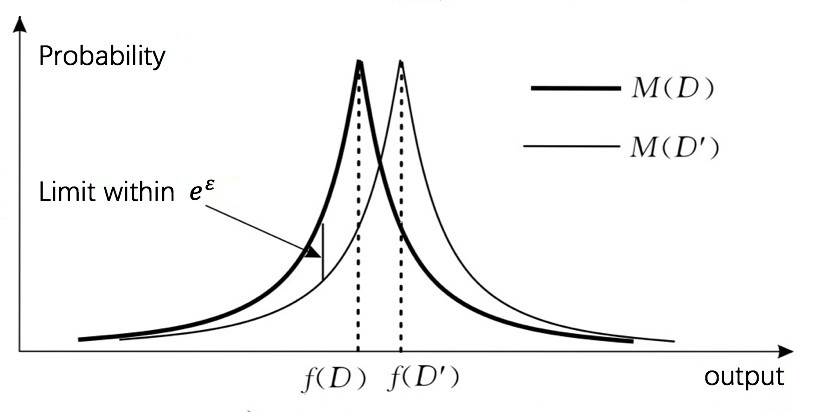
\includegraphics[scale=0.3]{varepsilon.png}
    %\vspace{-0.1cm}
    \caption{The output probability of random algorithms on adjacent datasets}
    \label{fig:figere}
    %\vspace{-0.2cm}
\end{figure}


For example, table 1 shows a medical dataset D, each of which indicates whether a person is suffering from cancer. The dataset provides a user with a statistical query service, but does not disclose the value of a specific record. Set the user input parameter $S_i$ and call the query function $f(i)=count(i)$ to get the number of records that satisfy the "diagnostic result" =1 before the I row in the dataset, and feedback the value of the function to the user. Suppose an attacker wants to speculate whether Alice has cancer and knows that Alice is in the fifth line of the data set, so it can be used $count(5) - count(4)$ to bring out the correct results.

\begin{table}[!htbp]
  \centering
  \caption{\label{tab:test}medical dataset}
  \begin{tabularx}
	\toprule
	 name & result\\
	\midrule
	 Tom & 0    \\
     Diego & 1  \\
     Jack & 1   \\
     Henry & 0  \\
     Alice & 1  \\
	\bottomrule
  \end{tabularx}
\end{table}


However, if $f$ is a query function that provides an $\varepsilon$-differential privacy protection, for example $f(i)=count(i)+noise$, noise is a random distribution of noise. Assuming that the possible output of $f(5)$ comes from the set \{2, 2.5, 3\}, then $f(5)$ will also output almost any possible value in the set \{2, 2.5, 3\} at almost exactly the same probability. So the attacker cannot get the desired results through $f(5)-f(4)$. This randomization method for statistical output makes it impossible for the attacker to get the difference between the query results, thus ensuring the security of each individual in the dataset.

From definition 1, it can be seen that the privacy protection budget $\varepsilon $ is used to control the probability ratio that the algorithm M obtains the same output on two adjacent data sets, which in fact reflects the level of privacy protection that M can provide. In practical applications, $\varepsilon $ usually take a very small value, such as 0.01, 0.1, or $ln2$, $ln3$, etc. The smaller the $\varepsilon $, the higher the level of privacy protection. When $\varepsilon $ is equal to 0, the protection level reaches the highest. At this time, for any adjacent data set, the algorithm  will output exactly the same result of the two probability distributions, these results can not reflect any useful information about the data set. Therefore, the value of ε should be combined with the specific requirements to achieve the balance of the security and availability of the output results.

\subsection{Sensitivity}

Differential privacy protection can be achieved by adding appropriate amount of interfering noise to the return value of the query function. Adding too much noise will affect the availability of the result. Too little noise will not provide enough security. Sensitivity is the key to determining the amount of noise to be added. The parameter, which refers to the deletion of any record in the data set caused by the largest change in the query results. In the differential privacy protection method defines two kinds of sensitivity, namely Global Sensitivity and Local Sensitivity .

\begin{definition}
[Global Sensitivity\cite{Nissim2007Smooth}] For $f$ : $D_{n}\rightarrow R^{d}$, the global sensitivity of $f$ is
\begin{equation}
G{S_f} = \mathop {\max }\limits_{x,y:d(x,y)=1}||f(x)-f(y)||
\end{equation}
\end{definition}

The global sensitivity of a function is determined by the function itself, and the different functions have different global sensitivity. Some functions have a small global sensitivity (such as the count function, its global sensitivity is 1), so only a small amount of noise can be added to cover up the result of a record being deleted. Differential privacy protection is realized, but for some functions, such as the average value and the median, it often has a larger global sensitivity.

When the global sensitivity is large, it is necessary to add enough noise to the output of the function to ensure privacy and result in poor data availability. Defines local sensitivity and other concepts related to its computation.

\begin{definition}
[Local Sensitivity\cite{Nissim2007Smooth}]For f : $D_{n}\rightarrow R^{d}$ and $x\in D^{n}$ the local sensitivity of f is
\begin{equation}
L{S_f} = \mathop {\max }\limits_{x,y:d(x,y)=1}||f(x)-f(y)||
\end{equation}
\end{definition}


The local sensitivity is determined by the function $f$ and the specific data in the given data set D. Due to the data distribution characteristics of the data set, the local sensitivity is usually much smaller than the global sensitivity. In addition, the relationship between local sensitivity and global sensitivity can be expressed as
\begin{equation}
G{S_f} = \mathop {\max }\limits_D (L{S_f}(D))
\end{equation}

However, because the local sensitivity reflects the data distribution characteristics of the data set to some extent, if the local sensitivity is directly used to calculate the noise amount, the sensitive information in the data set will be leaked. Therefore, the smooth upper bound is used together with local sensitivity to determine the amount of noise.

\begin{definition}
[mooth upper bound\cite{Dwork2011A}]Local sensitivity $L{S_f}(D)$, for any of the neighboring datasets D and $D′$ and $\beta > 0$, if function S satisfies $S(D) \ge L{S_f}(D)$ and $S(D) \le {e^\beta }S(D')$, then we call S the local sensitivity $β$-smooth upper bound of function $f$.
\end{definition}

All functions that satisfy this definition can be defined as a smooth upper bound, and a smooth sensitivity can be obtained by replacing the local sensitivity into the function, and then used to calculate the size of the noise. The relationship between the smooth upper bound and the local sensitivity, as shown in Figure 2.

\begin{figure}[h]
    \centering
    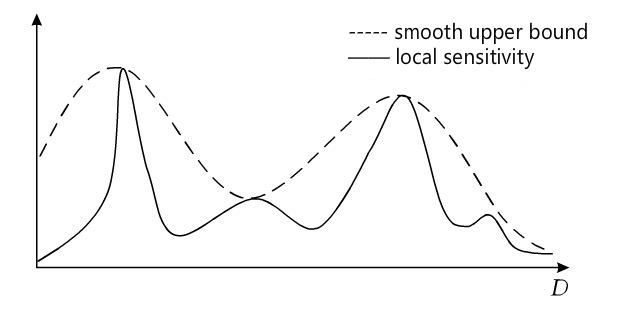
\includegraphics[scale=0.4]{smoothUpperBound.png}
    %\vspace{-0.1cm}
    \caption{Smooth upper bound}
    \label{fig:figere}
    %\vspace{-0.2cm}
\end{figure}


\begin{definition}
[Smooth sensitivity\cite{Nissim2007Smooth}] Given dataset D and $D'$,the function $S_{f,\beta }(D)=\mathop {\max }\limits_{D'}(LS_{f}(D')×e^{-\beta |D\Delta D'|})$ is called the $\beta$-smooth sensitivity of $f$, in which $\beta>0$.
\end{definition}

\subsection{Combination of Differentially Private Mechanisms}


\begin{theorem}[Parallel Theorem\cite{Mcsherry2010Privacy}]
Suppose we have a set of privacy mechanisms $M = \{ {M_1}, \ldots ,{M_m}\} $, if each ${M_i}$ provides ${\varepsilon _i}$-privacy guarantee on a disjointed subset of the entire dataset, M will provide $(\max \{ {\varepsilon _1}, \ldots ,{\varepsilon _m}\}) $-differential privacy. The parallel theorem
corresponds to a case where each ${M_i}$ is applied on disjointed subsets of the dataset. The ultimate privacy guarantee only depends on the largest privacy budget allocated to ${M_i}$.
\end{theorem} 


\begin{theorem}[Sequential Theorem\cite{Mcsherry2010Privacy}]
Suppose a set of privacy mechanisms $M = \{ {M_1}, \ldots ,{M_m}\} $, if each ${M_i}$ are sequentially performed on a dataset, and each ${M_i}$ provides ${\varepsilon _i}$ privacy guarantee, M will provide $(\sum\nolimits_{i = 1}^m \varepsilon  )$-differential privacy.
\end{theorem} 


\subsection{The Laplacian Mechanism}

The Laplace mechanism implements $\varepsilon$ differential privacy protection by adding random noise obeying the Laplace distribution to the exact query results. The location parameter is 0 and the Laplace of the scale parameter B is $Lap(b)$, then its probability density function is
\begin{equation}
p(x) = \frac{1}{{2b}}\exp ( - \frac{{|x|}}{b})
\end{equation}

\begin{definition} [laplace machanism\cite{Dwork2006Calibrating}]
A given set of data sets, D, has a function $f:D\rightarrow R^{d}$, whose sensitivity is  $\Delta f$, then the random algorithm $M(D)=f(D)+Y$ provides epsilon differential privacy protection, and $Y~\mathit{Lap}(\Delta f/\varepsilon )$ is random noise and obeys the scale parameter for the delta distribution.
\end{definition}

\begin{figure}[h]
    \centering
    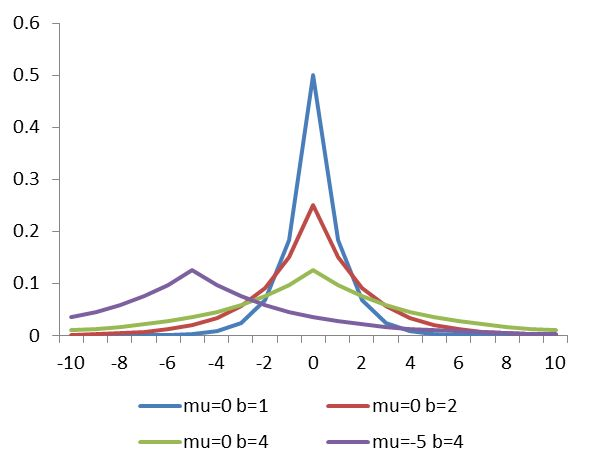
\includegraphics[scale=0.6]{laplace.png}
    %\vspace{-0.1cm}
    \caption{Laplace machanism}
    \label{fig:figere}
    %\vspace{-0.2cm}
\end{figure}

From the Laplace distribution of different parameters (Fig. 1), we can see that the smaller the $\varepsilon$, the greater the noise introduced.


\subsection{The Exponential Mechanism}

Since the Laplace mechanism is only suitable for numerical query results, in many practical applications, query results are entity objects (such as a scheme or a choice). In this case, McSherry and others have proposed an exponential mechanism.

The output domain of a query function is Range, and each value $r\in Range$ is an entity object. Under the exponential mechanism, the function $q(D,r)\rightarrow R$ is called the availability function of the output value r, which is used to evaluate the degree of the output value r.

\begin{definition}[exponential machanism\cite{Mcsherry2007Mechanism}]
The random algorithm M is input to the data set D, the output is an entity object $r\in Range$, the $q(D,r)$ is the availability function, and the $\Delta q$ is the sensitivity of the function $q(D,r)$. If the algorithm M is selected and output from the probability of the $exp(\frac{\varepsilon q(D,r) }{2\Delta q})$, the algorithm provides $\varepsilon$-differential privacy protection.
\end{definition}



\section{Machine Learning}
In machine learning, tasks are generally classified into broad categories. These categories are based on how learning is received or how feedback on the learning is given to the system developed.

Two of the most widely adopted machine learning methods are supervised learning which trains algorithms based on example input and output data that is labeled by humans, and unsupervised learning which provides the algorithm with no labeled data in order to allow it to find structure within its input data. In supervised learning, the computer is provided with example inputs that are labeled with their desired outputs. The purpose of this method is for the algorithm to be able to “learn” by comparing its actual output with the “taught” outputs to find errors, and modify the model accordingly. Supervised learning therefore uses patterns to predict label values on additional unlabeled data.In unsupervised learning, data is unlabeled, so the learning algorithm is left to find commonalities among its input data. As unlabeled data are more abundant than labeled data, machine learning methods that facilitate unsupervised learning are particularly valuable.

We will discuss the differential privacy protection methods in supervised learning and unsupervised learning respectively.




\subsection{Differentially Private Supervised Learning
}

\subsubsection{Naive Bayes Model}

In \cite{Barthe2016Differentially},they present PrivInfer, an expressive framework for writing and verifying differentially private Bayesian machine learning algorithms. Their framework allows to write data analysis as functional programs for Bayesian inference and to add noise to them in different ways using different metrics.They explore three ways to ensure differential privacy: by adding noise on the input, by adding noise on the output parameters based on p-norms, and by adding noise on the output parameters based on f-divergences.


In \cite{Li2018Differentially},they propose a novel privacy- preserving Naive Bayes learning scheme to handle the situation that the data owner not entirely trust each other.They point out that training sample always collected from multiple owner instead of a single data source.In this assumption,owners are not trust each other, which means they all intend to reveal sensitive data of others and protect their own privacy.To solve the problem above,they propose a privacy-preserving machine learning scheme in the multi-owner setting for a simple but highly effective classification, the Naive Bayes (NB) classification. The NB classifier model could meet the requirements of ε-differential privacy.

\subsubsection{Linear Regression}

In \cite{Wang2017Per},they present a new algorithm called AdaOPS which use the idea of Kifer et al. \cite{Kifer2013Private}, Blocki et al. \cite{Kenthapadi2012Privacy}, Sheffet \cite{Sheffet2015Differentially} for analyzing other related differentially private algorithms.They only need $n\varepsilon ^{2}=o(1)$ to achieve asymptotic efficiency.


\subsubsection{Linear SVM}

\subsubsection{Logistic Regression}

\subsubsection{Kernel SVM}
In \cite{Rubinstein2009Learning},they present a pair of mechanisms for private SVM learning, each of which releases a classifier based on a privacy-sensitive database of training data. In each case they establish differential privacy of their mechanisms via the algorithmic stability of regularized ERM—a property that  for any delta, no mechanism can be simultaneously (epsilon,delta)-useful and beta-differentially private for small epsilon and small beta.


\subsubsection{Decision Tree Learning}
\cite{Fletcher2016Decision}

\subsection{Differentially Private Unsupervised Learning}


\subsubsection{K-means clustering}
\cite{Pinot2018Graph}

\subsection{Differentially Private Dimensionality Reduction}


\subsubsection{Feature Selection}


\section{Conclusion}
The conclusion goes here.




%\IEEEtriggeratref{37}
\bibliographystyle{IEEEtran}
%\balance
\bibliography{bibliography}




\end{document}
